\documentclass[11pt]{scrartcl}
\usepackage{polski}
\usepackage[polish]{babel}

\usepackage{graphicx, float, caption, subcaption, amsmath}
\usepackage{tabularx, multirow, hyperref, enumitem, listings}
%\usepackage{minted}

\usepackage{listings, xcolor}
\definecolor{md-black}{rgb}{0.12, 0.12, 0.12}
\definecolor{md-teal}{rgb}{0.38, 0.79, 0.69}
\definecolor{md-mauve}{rgb}{0.76, 0.52, 0.75}
\definecolor{md-green}{rgb}{0.13, 0.55, 0.13}
\definecolor{md-red}{rgb}{0.82, 0.10, 0.14}
\definecolor{md-purple}{rgb}{0.69, 0.33, 0.73}
\definecolor{md-orange}{rgb}{0.96, 0.42, 0.18}
\definecolor{md-gray}{rgb}{0.44, 0.46, 0.51}

\lstset{
    language=Python,
    basicstyle=\color{md-teal}\ttfamily,
    keywordstyle=\color{md-mauve},
    commentstyle=\color{md-green},
    stringstyle=\color{md-red},
    numbers=left,
    numberstyle=\small\color{md-gray}\ttfamily,
    stepnumber=1,
    numbersep=5pt,
    backgroundcolor=\color{md-black},
    showspaces=false,
    showstringspaces=false,
    showtabs=false,
    frame=none,
    tabsize=4,
    captionpos=b,
    breaklines=true,
    breakatwhitespace=false,
    escapeinside={\%*}{*)},
    numbersep=-10pt,
    morekeywords={as}
}

\graphicspath{{images/}}

\title{Laboratorium 3 - Interpolacja}
\author{Mateusz Podmokły - II rok Informatyka WI}
\date{14 marzec 2024}

\begin{document}
    \maketitle

    \section{Treść zadania}
    \textbf{Zadanie 1.} Wyznacz wielomian interpolacyjny dla punktów
    reprezentujących populację Stanów Zjednoczonych na przestrzeni
    lat. Dane do interpolacji:

    \begin{table}[H]
        \centering
        \begin{tabular}{c | c}
            Rok & Populacja \\
            \hline
            1900 & 76 212 168 \\
            1910 & 92 228 496 \\
            1920 & 106 021 537 \\
            1930 & 123 202 624 \\
            1940 & 132 164 569 \\
            1950 & 151 325 798 \\
            1960 & 179 323 175 \\
            1970 & 203 302 031 \\
            1980 & 226 542 199 \\
        \end{tabular}
    \end{table}
    \subsection*{}
    Rozważ następujące funkcje bazowe $\phi_j(t)$ dla wielomianu,
    gdzie $j=1, \ldots ,9$:
    \begin{align}
        & \phi_j(t) = t^{j-1} \\
        & \phi_j(t) = (t-1900)^{j-1} \\
        & \phi_j(t) = (t-1940)^{j-1} \\
        & \phi_j(t) = \left(\frac{t-1940}{40}\right)^{j-1}
    \end{align}

    \subsection*{}
    Dla najlepiej uwarunkowanej bazy wielomianów wyznacz wielomian
    interpolacyjny na trzy sposoby. Pierwszy polega na rozwiązaniu
    układu równań powstałego z macierzy Vandermonde'a i funkcji bazowych
    \[
        \begin{bmatrix}
            \phi_1(x_1) & \phi_2(x_1) & \phi_3(x_1) & \cdots &
            \phi_n(x_1) \\
            \phi_1(x_2) & \phi_2(x_2) & \phi_3(x_2) & \cdots &
            \phi_n(x_2) \\
            \vdots & \vdots & \vdots & \ddots & \vdots \\
            \phi_1(x_n) & \phi_2(x_n) & \phi_3(x_n) & \cdots &
            \phi_n(x_n)
        \end{bmatrix}
        \begin{bmatrix}
            a_1 \\
            a_2 \\
            \vdots \\
            a_n
        \end{bmatrix}
        =
        \begin{bmatrix}
            y_1 \\
            y_2 \\
            \vdots \\
            y_n
        \end{bmatrix}
    \]

    \subsection*{}
    Następnie oblicz wielomian interpolacyjny Lagrange'a oraz wielomian
    interpolacyjny Newtona i dokonaj ekstrapolacji wielomianu do
    roku 1990. Porównaj otrzymaną wartość ekstrapolacji z prawdziwą
    wartością populacji w roku 1990 wynoszącą 248 709 873 \\
    Na koniec zaokrąglij dane wejściowe do pełnych milionów, ponownie
    oblicz współczynniki wielomianu i porównaj wyniki interpolacji
    z poprzednimi wynikami.

    \section{Specyfikacja użytego środowiska}
    Specyfikacja:

    \begin{itemize}
        \item Środowisko: Visual Studio Code,
        \item Język programowania: Python,
        \item System operacyjny: Microsoft Windows 11,
        \item Architektura systemu: x64.
    \end{itemize}

    \section{Rozwiązanie problemu}

    W realizacji rozwiązania wykorzystane zostały następujące biblioteki:
    \begin{lstlisting}
        import numpy as np
        import matplotlib.pyplot as plt
    \end{lstlisting}

    \subsection*{}
    Dla każdej funkcji bazowej wyznaczona została macierz Vandrmonde'a z użyciem
    funkcji \texttt{np.vander}, a następnie, dla każdej macierzy, współczynniki
    uwarunkowania macierzy funkcją \texttt{np.linalg.cond}. Najlepiej uwarunkowana
    okazała się macierz zbudowana z czwartego zbioru funkcji bazowych, więc ona
    została użyta do interpolacji. Dokonana została ekstrapolacja wielomianu do
    roku 1990. \\
    Obliczenie współczynników wielomianu:
    \[
        \texttt{np.linalg.solve(V,y)}
    \]
    Obliczamy wielomian interpolacyjny Lagrange'a ze wzoru
    \[
        w(x)=\sum_{i=0}^{n}y_i \cdot \prod_{j=0 \land j \neq i}^{n}
        \frac{x-x_j}{x_i-x_j}
    \]
    oraz wielomian interpolacyjny Newtona
    \[
        w(x)=a_0+ \sum_{i=1}^{n} a_i \prod_{j=0}^{i-1} (x-x_j)
    \]
    współczynniki $a_0,a_1, \ldots ,a_n$ są kolejnymi elementami na przekątnej
    macierzy
    \[
        \begin{bmatrix}
            f(x_0) \\
            f(x_1) & f[x_0,x_1] \\
            f(x_2) & f[x_1,x_2] & f[x_0,x_1,x_2] \\
            \vdots & \vdots & \vdots & \ddots \\
            f(x_n) & f[x_{n-1},x_n] & f[x_{n-2},x_{n-1},x_n] & \cdots &
            f[x_0, \ldots ,x_n] \\
        \end{bmatrix}
    \]
    gdzie $f[x_0,x_1, \ldots ,x_k]$ to różnica dzielona zdefiniowana następująco
    
    \begin{align*}
        & f[x_i] = f(x_i) \\
        & f[x_i, \ldots ,x_{i+j+1}] =
        \frac{f[x_{i+1}, \ldots ,x_{i+j+1}]-f[x_i, \ldots ,x_{i+j}]}{x_{i+j+1}-x_i}
    \end{align*}
    Wartości wielomianu zostały obliczone z odstępami jednorocznymi. Następnie
    zaokrąglowo dane zawierające wartości populacji do pełnych milionów
    i ponownie wyznaczono macierze oraz współczynniki wielomianu.

    \section{Przedstawienie wyników}
    \subsection{Interpolacja}
    Współczynniki uwarunkowania czterech macierzy:
    \begin{align*}
        cond_1 &= 8.49 \cdot 10^{41} \\
        cond_2 &= 5.99 \cdot 10^{15} \\
        cond_3 &= 9.32 \cdot 10^{12} \\
        cond_4 &= 1.61 \cdot 10^3
    \end{align*}
    Najlepiej uwarunkowana macierz to macierz 4.

    \begin{figure}[H]
        \centering
        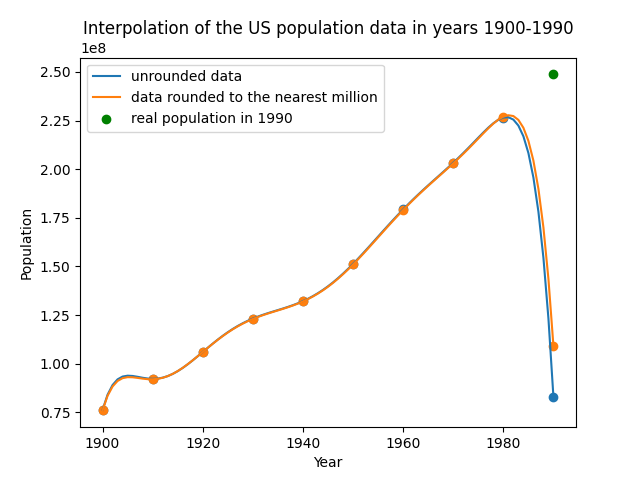
\includegraphics[width=0.8\linewidth]{interpolation.png}
        \caption{Porównanie uzyskanych interpolacji.}
    \end{figure}

    \subsection*{}
    Różnice między interpolacją uogólnionym wielomianem, interpolacją Lagrange'a
    i interpolacją Newtona są niewielkie i niezauważalne na wykresie. Jedynie
    zaokrąglenie danych wejściowych do pełnych milionów powoduje niewielką zmianę
    wielomianu.

    \subsection{Ekstrapolacja}
    Prawdziwa wartość dla roku 1990: 248 709 873.

    \subsubsection*{Przed zaokrągleniem danych}
    Wartość uzyskana z ekstrapolacji: 82 749 141. \\
    Błąd względny uzyskanej wartości: 66.73\%.

    \subsubsection*{Po zaokrągleniu danych do pełnych milionów}
    Wartość uzyskana z ekstrapolacji: 109 000 000. \\
    Błąd względny uzyskanej wartości: 56.17\%.

    \section{Wnioski}

\end{document}
